\documentclass[a4paper]{article}
\usepackage{graphicx}
\usepackage{fullpage} % Package to use full page
\usepackage{color}

\usepackage{listings}
\lstset{ 
	language=Matlab,                		% choose the language of the code
%	basicstyle=10pt,       				% the size of the fonts that are used for the code
	numbers=left,                  			% where to put the line-numbers
	numberstyle=\footnotesize,      		% the size of the fonts that are used for the line-numbers
	stepnumber=1,                   			% the step between two line-numbers. If it's 1 each line will be numbered
	numbersep=5pt,                  		% how far the line-numbers are from the code
%	backgroundcolor=\color{white},  	% choose the background color. You must add \usepackage{color}
	showspaces=false,               		% show spaces adding particular underscores
	showstringspaces=false,         		% underline spaces within strings
	showtabs=false,                 			% show tabs within strings adding particular underscores
%	frame=single,	                			% adds a frame around the code
%	tabsize=2,                				% sets default tabsize to 2 spaces
%	captionpos=b,                   			% sets the caption-position to bottom
	breaklines=true,                			% sets automatic line breaking
	breakatwhitespace=false,        		% sets if automatic breaks should only happen at whitespace
	escapeinside={\%*}{*)}          		% if you want to add a comment within your code
}

\author{Ryan Day}
\title{Optimization Homework 3}
\date{February 11, 2019}

\begin{document}
    \maketitle
    \tableofcontents
    \newpage
    \section{Written description of program}
    I implemented Steepest Descent and also the Quasi-Newton method with a BFGS update. 
    I used recursion to call the line updates so that I wouldn't have to fiddle around with while or for loops.
    
    The line search was implemented by first taking a step in the search direction as calculated by the chosen algorithm with $\alpha = 0.7$.
    If this step is too big, the program will start the line search over from the starting point and use $\alpha_{current}/100$.
    This will keep happening until the first step is smaller than the initial value. 
    After this, the line search keeps searching by doubling alpha each step, always from the same starting point. 
    Once the value of the alpha is bigger than the alpha of the previous value, it finds the value of the point at $\alpha_{current}*0.75$, halfway between the last point and the second to last point.
    It then takes the minimum point and the two points around that one, does a quadratic fit, and finds the alpha of the minimum function value of that fit.
    It then takes a step and finds a new x0, and checks the gradient at this point. 
    It repeats this process again until each component of the gradient is under the specified tolerance.
    \section{Did the methods perform as well as I expected?}    
    For the quadratic equation, the Quasi-Newton algorithm converged with three line searches, which is exactly what we would predict with 3 variables.
    We know that since Quasi-Newton approximates the algorithm as a quadratic, if the function is a quadratic then it will converge very quickly.
    Steepest Descent converged in 21 line searches, which is fine. This wass not as good as Quasi-Newton, but the function was not elliptical enough to cause the algorithm to take a while to converge.
    
    For the Rosenbrock function, Steepest Descent oscillated back in forth as seen in the figure on page 5. 
    This is predictable because it always tries to go to the minimum but it overshoots it.
    The Quasi-Newton method had some erratic behavior but converged pretty quickly. 
    \newpage
    \section{Test Results Quadratic function}
        \subsection{Results for Quasi-Newton Method}
            
            \begin{tabular}{|l|l|l|l|l|l|}
            \hline
              & Starting Point                                                    & Function Value & Search Direction                                                      & Step Length & Nobj for search \\
              \hline
            1 & \begin{tabular}[c]{@{}l@{}}10\\ 10\\ 10\end{tabular}              & 520            & \begin{tabular}[c]{@{}l@{}}-0.99426\\ 0.06414\\ -0.08552\end{tabular} & 7.8185      & 7               \\
                \hline
            2 & \begin{tabular}[c]{@{}l@{}}2.226\\ 10.502\\ 9.3313\end{tabular}   & 154.343        & \begin{tabular}[c]{@{}l@{}}-0.1624\\ -0.5596\\ -0.8362\end{tabular}   & 18.3067     & 9               \\
                \hline
            3 & \begin{tabular}[c]{@{}l@{}}-0.7467\\ 0.2560\\ -5.977\end{tabular} & -14.399        & \begin{tabular}[c]{@{}l@{}}0.05846\\ 0.66920\\ -0.78849\end{tabular}  & 3.270       & 6               \\
                \hline
            4 & \begin{tabular}[c]{@{}l@{}}-0.5556\\2.4444\\-8.5556\end{tabular}                                            & -22.3889       &                                                                       &             & 1 \\
            \hline
            \end{tabular}

            TOTAL OBJ CALLS = 23

            TOTAL GRAD CALLS = 4

        \subsection{First five steps for Steepest Descent}
            \begin{tabular}{|l|l|l|l|l|l|}
            \hline
              & Starting Point                                                    & Function Value & Search Direction                                                      & Step Length & Nobj for search \\ \hline
            1 & \begin{tabular}[c]{@{}l@{}}10\\ 10\\ 10\end{tabular}              & 520            & \begin{tabular}[c]{@{}l@{}}-0.99426\\ 0.06414\\ -0.08552\end{tabular} & 7.8185      & 7               \\ \hline
            2 & \begin{tabular}[c]{@{}l@{}}2.226\\ 10.502\\ 9.3313\end{tabular}   & 154.3          & \begin{tabular}[c]{@{}l@{}}0.0335\\ -0.5723\\ -0.8194\end{tabular}    & 12.5261     & 8               \\ \hline
            3 & \begin{tabular}[c]{@{}l@{}}2.6466\\ 3.3328\\ -0.9320\end{tabular} & 38.88          & \begin{tabular}[c]{@{}l@{}}-0.9765\\ 0.1557\\ -0.1487\end{tabular}    & 2.5121      & 6               \\ \hline
            4 & \begin{tabular}[c]{@{}l@{}}0.1934\\ 3.7239\\ -1.3057\end{tabular} & 1.5472         & \begin{tabular}[c]{@{}l@{}}0.1236\\ -0.1598\\ -0.9793\end{tabular}    & 4.3808      & 7               \\ \hline
            5 & \begin{tabular}[c]{@{}l@{}}0.7352\\ 3.0236\\ -5.5961\end{tabular} & -12.99         & \begin{tabular}[c]{@{}l@{}}-0.9819\\ 0.1229\\ -0.1441\end{tabular}    & 0.9798      & 4               \\ \hline
            \end{tabular}

            TOTAL OBJ CALLS = 166

            TOTAL GRAD CALLS = 24
    \newpage
    \section{Test Results Rosenbrocks function}
        \subsection{Results for Quasi-Newton Method} 
        TOTAL OBJ CALLS = 162,
        TOTAL GRAD CALLS = 22
        \begin{center}
            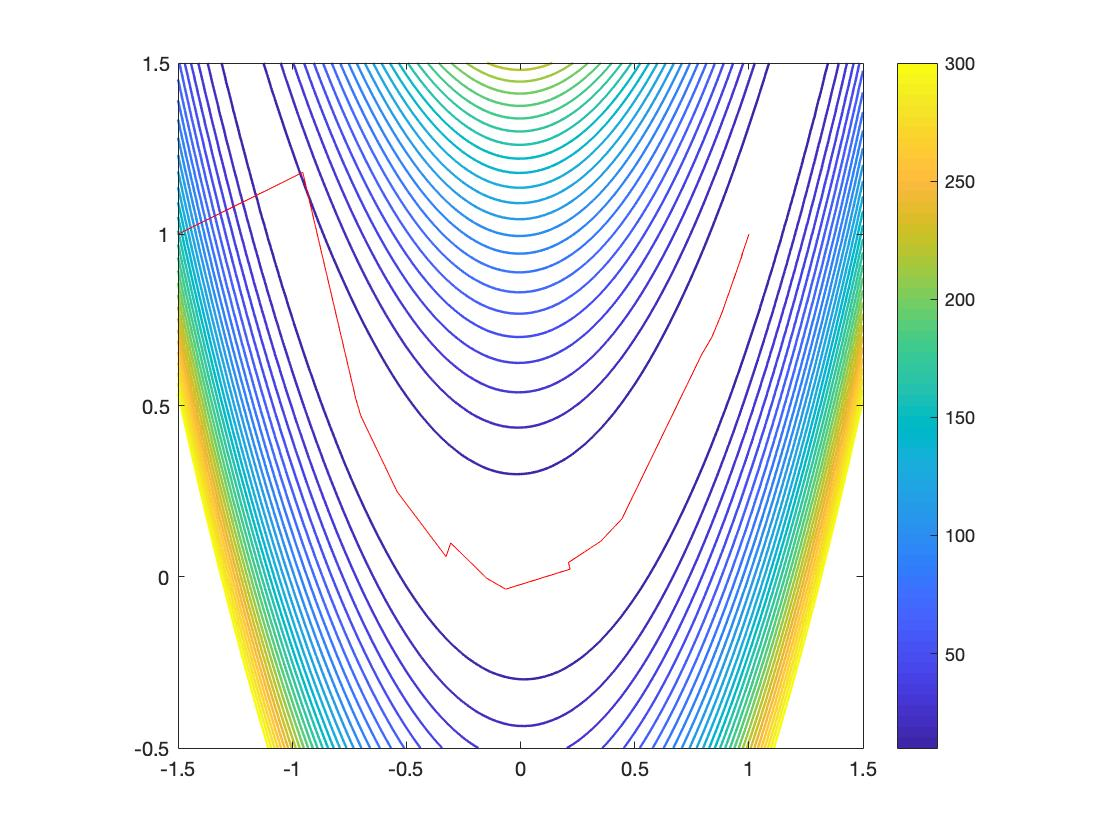
\includegraphics[scale = 0.32]{images/QNRosenbrock.jpg}
        \end{center}   
        \subsection{First 100 Steps for Steepest Descent}       
        TOTAL OBJ CALLS TO CONVERGE = 3931,
        TOTAL GRAD CALLS TO CONVERGE = 559
        \begin{center}
            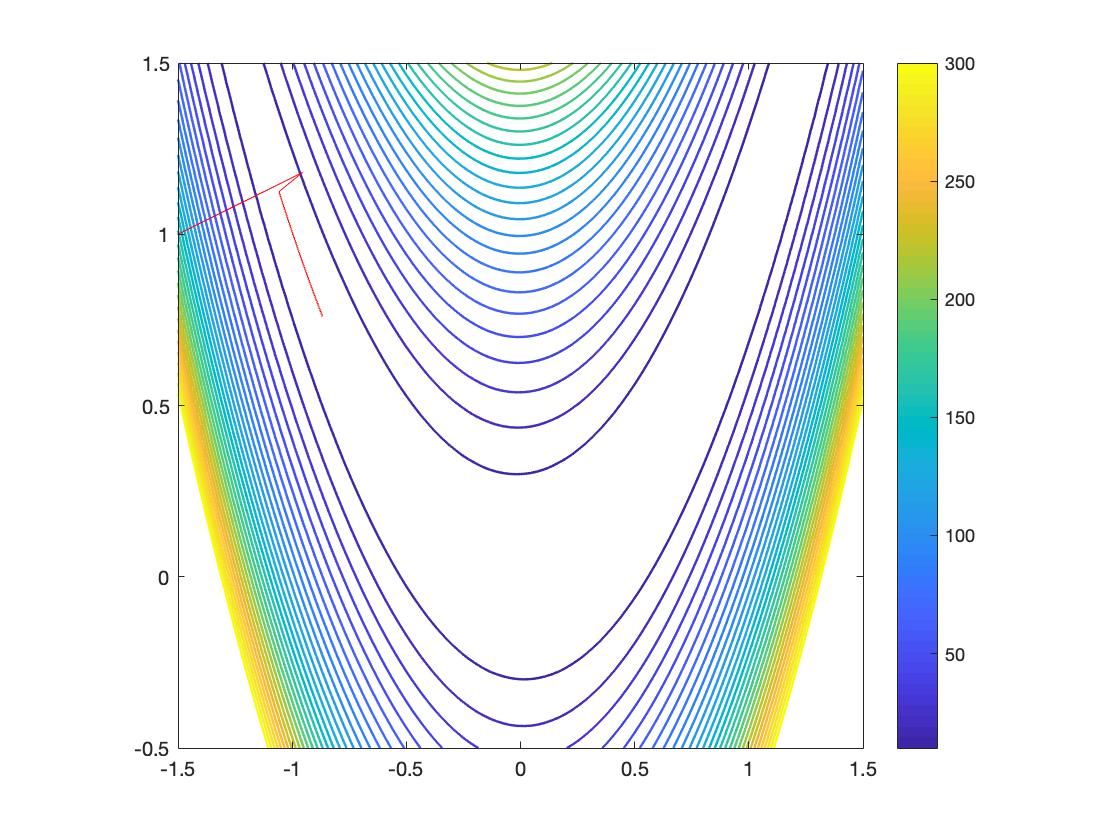
\includegraphics[scale=0.3]{images/SDRosenbrock.jpg}
        \end{center}
        Although its hard to see here, the algorithm is taking lots of tiny steps around the line. 
        In the zoomed up view you can see a very small zig zag pattern.
        \begin{center}
            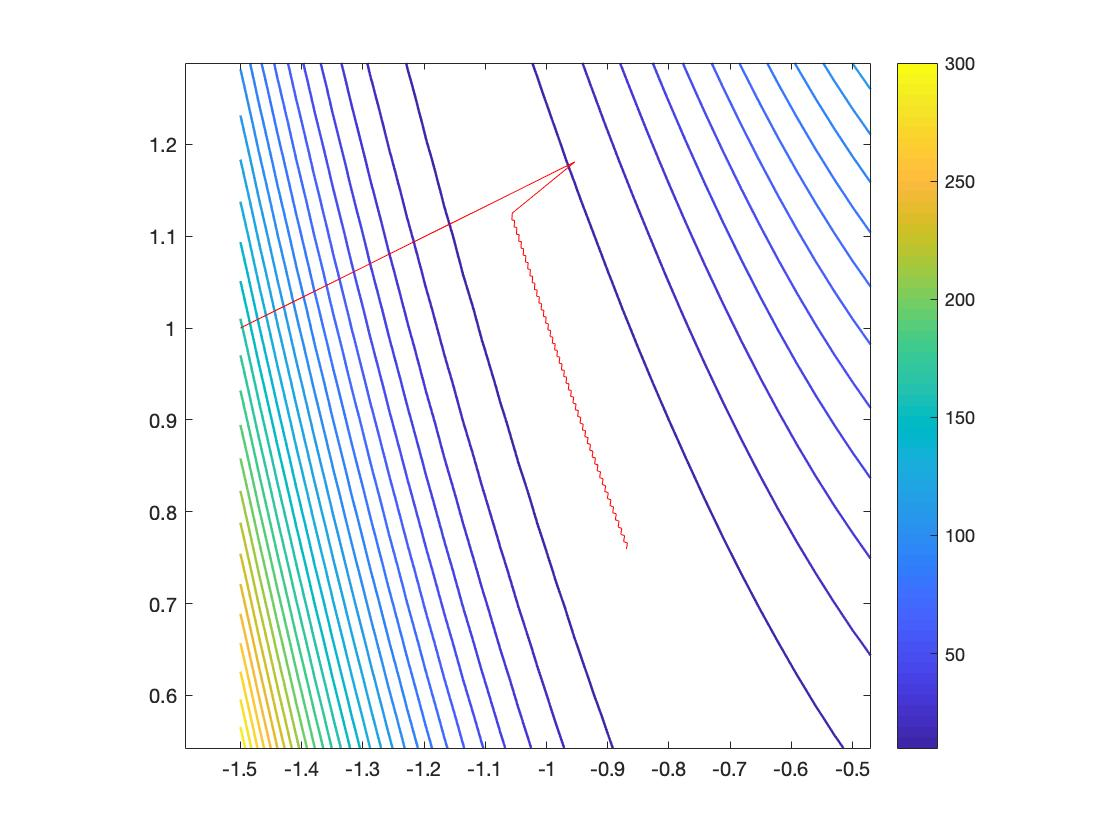
\includegraphics[scale=0.45]{images/closeup.jpg}
        \end{center}
        \section{Code}
        \subsection{fminun}
        \lstinputlisting[language=Matlab]{../fminun.m}
        \subsection{fminunDriver}
        \lstinputlisting[language=Matlab]{../fminunDrivHw.m}
        \newpage
        \subsection{Rosenbrock Contour plot}
        \lstinputlisting[language=Matlab]{../ContourPlotRosenbrock.m}



\end{document}